\documentclass[12pt]{article}
\usepackage[left=2.50cm,right=2.50cm,top=2.50cm,bottom=2.50cm]{geometry}
\geometry{a4paper}
\usepackage{fancyhdr}
\pagestyle{fancy}
\usepackage[T1]{fontenc}
\usepackage[utf8]{inputenc}
\usepackage{mathpazo} % Cool type
%\usepackage[
%	backend=biber,
%	style=authoryear,
%	%language=autobib,
%	%sortlocale=en_US,
%	%natbib=true,
%	url=false,
%	doi=true,
%	%eprint=false,
%	hyperref=auto
%]{biblatex}
\usepackage[
	authordate,
	backend=biber
]{biblatex-chicago}
\DeclareFieldFormat[article,book,inproceedings]{title}{#1}
\bibliography{biblio.bib}
%\addbibresource{biblio.bib}
\usepackage[running]{lineno}
\usepackage{enumitem}
\usepackage{color}
\usepackage{graphicx}
%\usepackage[foot]{amsaddr}
\usepackage{setspace}
\usepackage{amsthm,amsmath,amsfonts,amssymb}
\usepackage{pdfpages}
\usepackage{todonotes}
\usepackage{url}            % simple URL typesetting
\usepackage{nicefrac}       % compact symbols for 1/2, etc.
\usepackage{microtype}      % microtypography
%\usepackage{doi}
\usepackage{tabularx, array, booktabs, caption, subcaption, pdflscape, makecell, siunitx, multirow, ragged2e}
% Embed files inside the PDF
\usepackage{embedfile}
\usepackage{xcolor}
% Define the color for links
%\definecolor{mylinkcolor}{RGB}{0, 0, 255}
\usepackage[
	colorlinks=true,
	linkcolor=purple,
	citecolor=blue,
	urlcolor=cyan,
	bookmarks=true,
	hypertexnames=true
]{hyperref}
\hypersetup{
	bookmarksnumbered=true,
	bookmarksopen=true,
}
%\onehalfspacing
%\renewcommand\refname{\textsc{Literature Cited}}

\usepackage{sectsty}
\sectionfont{\centering}
\subsectionfont{\centering}
\subsubsectionfont{\centering}

\AtEveryBibitem{\clearfield{month}}
\AtEveryBibitem{\clearfield{day}}

% This is for the ORCID
\usepackage{academicons}
\definecolor{orcidlogocol}{HTML}{A6CE39}
\usepackage{orcidlink}

\newtheorem{theorem}{Theorem}
\newtheorem{acknowledgement}[theorem]{Acknowledgement}
\newtheorem{algorithm}[theorem]{Algorithm}
\newtheorem{axiom}[theorem]{Axiom}
\newtheorem{case}[theorem]{Case}
\newtheorem{claim}[theorem]{Claim}
\newtheorem{conclusion}[theorem]{Conclusion}
\newtheorem{condition}[theorem]{Condition}
\newtheorem{conjecture}[theorem]{Conjecture}
\newtheorem{corollary}[theorem]{Corollary}
\newtheorem{criterion}[theorem]{Criterion}
\newtheorem{definition}[theorem]{Definition}
\newtheorem{example}[theorem]{Example}
\newtheorem{exercise}[theorem]{Exercise}
\newtheorem{lemma}[theorem]{Lemma}
\newtheorem{notation}[theorem]{Notation}
\newtheorem{Question}[theorem]{Question}
\newtheorem{problem}[theorem]{Problem}
\newtheorem{proposition}[theorem]{Proposition}
\newtheorem{remark}[theorem]{Remark}
\newtheorem{solution}[theorem]{Solution}
\newtheorem{summary}[theorem]{Summary}
\newtheorem{fact}[theorem]{Fact}
\newcommand{\cqd}{\hfill \rule{5pt}{5pt}}
\def \N{\mathbb{N}}
\linespread{1.2}

\def\essinf{\mathop{\textrm{ess\,inf}}}
\def\esssup{\mathop{\textrm{ess\,sup}}}
\def\eps{\varepsilon}
\def\vp{\varphi}
\def\vt{\vartheta}
\def\vr{\varrho}
\def\lra{\longrightarrow}
\def\lraw{\stackrel{w}{\longrightarrow}}
\def\lraws{\stackrel{w^*}{\longrightarrow}}
\def\lms{\longmapsto}
\def\wh{\widehat}
\def\wt{\widetilde}
\def\ol{\overline}
\def\qfa{\quad\forall}
\def\qaq{\quad\textrm{and}\quad}
\def\qwith{\quad\textrm{with}\ }
\def\qin{\quad\textrm{in}\ }
\def\qor{\quad\textrm{or}\ }
\def\qon{\quad\textrm{on}\ }
\def\qas{\quad\textrm{as}\ }
\def\pO{\partial\Omega}
\def\oO{\overline{\Omega}}
\def\oirn{\Omega\subseteq\mathbb{R}^N}
\def\rr{\mathbb{R}}
\def\nn{\mathbb{N}}
\def\divv{\mathrm{div}\,}
\def\zio{z\in\Omega}
\def\io{\int_{\Omega}}
\def\calA{\mathcal{A}}
\def\calF{\mathcal{F}}
\def\calL{\mathcal{L}}
\def\dom{\mathrm{dom}}
\def\limn{\lim_{n\rightarrow +\infty}}
\def\limsupn{\limsup\limits_{n\rightarrow +\infty}}
\def\liminfn{\liminf\limits_{n\rightarrow +\infty}}

\def\essinf{\mathop{\textrm{ess\,inf}}}
\def\esssup{\mathop{\textrm{ess\,sup}}}
\def\eps{\varepsilon}
\def\vp{\varphi}
\def\vt{\vartheta}
\def\vr{\varrho}
\def\lra{\longrightarrow}
\def\lraw{\stackrel{w}{\longrightarrow}}
\def\lraws{\stackrel{w^*}{\longrightarrow}}
\def\lms{\longmapsto}
\def\wh{\widehat}
\def\wt{\widetilde}
\def\ol{\overline}
\def\qfa{\quad\forall}
\def\qaq{\quad\textrm{and}\quad}
\def\qwith{\quad\textrm{with}\ }
\def\qin{\quad\textrm{in}\ }
\def\qor{\quad\textrm{or}\ }
\def\qon{\quad\textrm{on}\ }
\def\qas{\quad\textrm{as}\ }
\def\pO{\partial\Omega}
\def\oO{\overline{\Omega}}
\def\oirn{\Omega\subseteq\mathbb{R}^N}
\def\rr{\mathbb{R}}
\def\nn{\mathbb{N}}
\def\divv{\mathrm{div}\,}
\def\zio{z\in\Omega}
\def\io{\int_{\Omega}}
\def\calA{\mathcal{A}}
\def\calF{\mathcal{F}}
\def\calL{\mathcal{L}}
\def\dom{\mathrm{dom}}
\def\limn{\lim_{n\rightarrow +\infty}}
\def\limsupn{\limsup\limits_{n\rightarrow +\infty}}
\def\liminfn{\liminf\limits_{n\rightarrow +\infty}}

\newcommand{\R}{\mathbb{R}}
\newcommand{\E}{\mathbb{E}}
\newcommand{\Z}{\mathbb{Z}}
\newcommand{\I}{\mathbb{I}}

\newcommand{\slim}{\mathop{\mathrm{slim}}}
\newcommand{\hsd}{\mathop{\mathrm{dist}\,}}
\newcommand{\hd}{\mathop{\mathrm{dist}^*\,}}
\newcommand{\px}{\mathop{\mathcal{P}(X)}}

%\let\origmaketitle\maketitle
%\def\maketitle{
%	\begingroup
%	\def\uppercasenonmath##1{} % this disables uppercasing title
%	\let\MakeUppercase\relax % this disables uppercasing authors
%	\origmaketitle
%	\endgroup
%}

\title{\textbf{{\LARGE Catastrophic Bifurcation in the Dynamics of a Threatened Bird Community Triggered by a Planetary-Scale Environmental Perturbation}}}

\usepackage{authblk}

\author[a,b]{Pablo Almaraz\orcidlink{0000-0003-1416-2695}\thanks{Corresponding Author: Pablo Almaraz. E-mail: pablo.almaraz@csic.es}}
\author[c]{Andy J. Green}

\affil[a]{Departamento de Ecuaciones Diferenciales y Análisis Numérico, Facultad de Matemáticas, Universidad de Sevilla, Campus Reina Mercedes, 41012, Sevilla, Spain.}
\affil[b]{Grupo de Oceanografía de Ecosistemas, Instituto de Ciencias Marinas de Andalucía, CSIC, Puerto Real, 11519, Spain.}
\affil[c]{Departamento de Biología de la Conservación y Cambio Global, Estación Biológica de Doñana EBD-CSIC, Avda. Américo Vespucio 26, 41092, Sevilla, Spain.}

\renewcommand\Authfont{\small} % Tamaño de letra para nombres de autores
\renewcommand\Affilfont{\small} % Tamaño de letra para afiliaciones

%\renewcommand\Authands{ and }
\renewcommand\Authands{, }

\date{}
%\date{\today}
%\date{\textbf{Open Research statement}: Data, code, and scripts will be made available in Github and Zenodo upon acceptance. \\
%Received 9 February 2021\\Revised 26 August 2021\\Accepted 15 November 2021.\\
%Handling Editor: }

% Clear default header and footer styles
\fancyhf{}

% Define header style
\lhead{\leftmark} % Place the section name on the left
\rhead{\thepage}  % Place the page number on the right

% Alternate header with abbreviated manuscript title
\fancyhead[RO,LE]{\href{https://doi.org/10.1016/j.biocon.2024.110466}{Almaraz \& Green (2024)}}

% Set the top rule line
\renewcommand{\headrulewidth}{0.4pt}
% Set the bottom rule line in the footer
\renewcommand{\footrulewidth}{0.4pt}

% Define footer style with placeholders
%\lfoot{Almaraz and Green (2023)}  % Placeholder for authors
%\cfoot{} % Placeholder for journal
%\rfoot{Date: \today} % Placeholder for date
%\rfoot{Biological Conservation} % Placeholder for journal
\lfoot{\textit{Biological Conservation}: \href{https://www.sciencedirect.com/journal/biological-conservation/special-issue/10DNPT6S9QV}{'Non-equilibrium perspectives in biological conservation'}}
% Centered page number in the footer
%\fancyfoot[C]{\thepage}
\fancyfoot[R]{\thepage}

\makeatletter
\def\maxwidth{ %
	\ifdim\Gin@nat@width>\linewidth
	\linewidth
	\else
	\Gin@nat@width
	\fi
}
\makeatother

\usepackage{framed}
\makeatletter
\newenvironment{kframe}{%
	\def\at@end@of@kframe{}%
	\ifinner\ifhmode%
	\def\at@end@of@kframe{\end{minipage}}%
\begin{minipage}{\columnwidth}%
	\fi\fi%
	\def\FrameCommand##1{\hskip\@totalleftmargin \hskip-\fboxsep
		\colorbox{shadecolor}{##1}\hskip-\fboxsep
		% There is no \\@totalrightmargin, so:
		\hskip-\linewidth \hskip-\@totalleftmargin \hskip\columnwidth}%
	\MakeFramed {\advance\hsize-\width
		\@totalleftmargin\z@ \linewidth\hsize
		\@setminipage}}%
{\par\unskip\endMakeFramed%
	\at@end@of@kframe}
\makeatother

\begin{document}

\maketitle
%\thispagestyle{empty}


\newpage
%\setcounter{page}{1} % Reinicia el contador de página

\linenumbers

\begin{abstract}

\onehalfspacing

	Ecological modeling has been traditionally dominated by a focus on the asymptotic behavior, but transient dynamics can have a profound effect on species and community persistence. We show a strong non-stationary coupling of ecological drivers in one of the world's major Mediterranean ecosystems, Doñana wetlands, which is currently threatened by many stressors. Recurrent changes in precipitation fluctuations triggered sudden reorganizations in community trends and population dynamics of a guild of ten wintering waterfowl species during a 36-year period. An anomalously dry and cold transient period in the Northern Hemisphere induced by the volcanic eruption of Mt. Pinatubo in 1991, prompted an abrupt shift to an alternative regime of fluctuating species densities. Most species did not recover previous values even though local weather patterns and large-scale climatic conditions returned to normal values. Although the dynamical stability of the community is similar in both regimes, structural stability declined: the probability of feasibility dropped across time due to depressed population densities at equilibrium. A stochastic cusp catastrophe model fitted to the time series data suggests that the spatio-temporal persistence of cold and dry conditions in the wintering areas, coupled with warm and wet conditions in the breeding grounds, modulated local ecological conditions and induced hysteresis through behavioral shifts to alternative wintering sites. Our study provides empirical evidence for the existence of a catastrophic bifurcation triggered by a tipping point in the dynamics of an imperiled terrestrial vertebrate community, highlighting the relevance of history and multi-stability in explaining current patterns in biological conservation.\\

	\subsubsection*{Keywords} Alternative stable states; Doñana wetlands; Stochastic cusp catastrophe;p Tipping point; Transient dynamics; Volcanism..
	
\end{abstract}

\markboth{Abstract}{}
\addcontentsline{toc}{section}{Abstract}

\newpage

%\doublespacing
\onehalfspacing

\section*{Introduction}
\label{sec:Introduction}
\markboth{Introduction}{}
\addcontentsline{toc}{section}{Introduction}

The stability of populations and communities in response to environmental perturbations is currently one of the most relevant research topics in the field of global change ecology (\cite{Bjornstad2001,Post2013,Vellend2016,Yang2019}). Despite the early appreciation that ecosystems might operate under more than one stable state (e.g., \cite{Holling1973,May1976a}), the main focus of theoretical ecology is still dominated by the asymptotic stability of autonomous (time-independent) ecological models. However, a growing body of evidence suggests that many ecological systems might operate under nonlinear dynamics characterized by abrupt, transient shifts from one stable state to another, usually preceded by tipping points (\cite{Fukami2011,Petraitis2013,Yletyinen2016,Rocha2018,Clements2018a,Dakos2019,Chen2020a}). This behavior, commonly known as alternative stable states, is common in marine, freshwater, and terrestrial ecosystems (\cite{Steele1996,Knowlton2004,Capon2015,Gsell2016a}; review in \cite{Rocha2015}).\\

In global change scenarios, understanding this non-linear behaviour is a major research goal (\cite{Rockstrom2009,Barnosky2012,Steffen2015a,Nash2017}). Progress in this field has been largely limited by semantic and statistical confusions on the specific mechanisms, processes and patterns involved in the characterization of alternative stable states (\cite{Suding2004a,Capon2015,Kuiper2015}). A regime shift denotes a statistical change in the parameters forcing a system, while a phase transition alludes to a change in the state of some attribute of the system (\cite{Scheffer2009a}). From this it follows that regime shifts should usually translate to phase transitions, but the detection of the latter does not necessarily demonstrate the existence of the former (e.g., \cite{Rudnick2003}). Indeed, evaluating whether alternative states are stable is far from trivial (\cite{Scheffer2009a,Stelzer2021}). Alternative stable states give rise to hysteresis: under the same concurrent environmental conditions there may exist several stable states, and the location of the system in a particular state may be better explained by historical conditions than by present ones (\cite{Scheffer2009a,Clements2018a}).\\

The overall consequence of this is that the abrupt phase transitions detected within ecological time-series are not always explicitly linked to the regime shifts potentially triggering them, thus yielding a rather phenomenological understanding of alternative stable states and regime shifts (\cite{Hastings2004,Montoya2017,Hastings2018,Hillebrand2020a}). Thus, to date it is unclear how abrupt regime shifts at different levels of ecological organization are intertwined, and to what extent this non-linear behaviour stem from external disturbances or internal dynamics (\cite{Scheffer2009a}). For example, abrupt ecological disturbances have only recently been linked mechanistically to extreme climatic events, such as large volcanic eruptions and intense hurricanes (e.g., \cite{Kuhnt2005,Schoener2006,Vazquez-Loureiro2019,Osland2020}). In particular, volcanism is regarded as one of the major perturbations not only to planetary climate (\cite{Osipov2021,Millan2022}), but also to ecological systems at all organizational, temporal and spatial scales (\cite{Sadler1999,Oppenheimer2003,Crisafulli2015,Jiang2022,Green2022,Chen2022a,Cabon2022}). One of the most recent major volcanic eruptions was that of the Mount Pinatubo on Luzon Island, Philippines, in 1991. This eruption is classified by geologist as a colossal event, with a return time between 50 and 100 years (e.g., \cite{Labitzke1992,Robock2000}). After producing the largest stratospheric volcanic aerosol cloud of the 20th century, the climatic impacts of Mt. Pinatubo eruption were of a planetary scale and lasted for several years (\cite{McCormick1995,Robock2002,Douglass2005}). The Mt. Pinatubo eruption provided a natural experiment testing the response of the global atmosphere and biosphere to large geological phenomena (\cite{Soden2002,Church2005,Khodri2017,Booth2012}). Consequently, a suite of ecological effects of this transient major perturbation were detected in several world ecosystems (\cite{Genin1995,Lucht2002a,Gu2003,Kuhnt2005,Trenberth2007}). Nevertheless, by definition, the frequency of such events is rare, so there are few opportunities to study the effects of single major perturbations on ecological dynamics in the long-term, while accounting for system dynamics before and after the perturbation.\\

Using a 36-year (1978-2013) dataset of abundance fluctuations of a wintering waterfowl community, we provide evidence on the coupling of abrupt shifts in the environmental, anthropogenic and biological subcomponents in one of the largest and best preserved Mediterranean wetland ecosystems in the world (Doñana wetlands, SW Spain; \cite{Rendon2008,Almaraz2012,Green2018}). This major ecosystem, historically supporting more than 1 million wintering birds from breeding grounds across the Palaearctic, is a Biosphere Reserve and includes a UNESCO World Heritage site. In spite of this, it is currently considered under severe threat due to several anthropogenic stressors, mainly groundwater abstractions and greenhouse-based agriculture (\cite{Scheffer2015a,Green2017a,Green2018,Camacho2022,Santamaria2023,DeFelipe2023a}). Waterbird communities are particularly useful for time-series analysis, because their populations are relatively easy to count, and can act as useful bioindicators of wetland biodiversity (\cite{Green2014}). Previous analyses (\cite{Almaraz2012}) detected an abrupt shift in the wintering waterfowl community of Doñana wetlands synchronized with a climatically harsh period lasting from 1992 to 1995. This low population density regime apparently became permanent even though local weather conditions returned to normal values. This transient period, characterized by anomalously dry and cold wintering seasons, is linked to the injection of massive amounts of sulfate aerosols by the eruption of Mt. Pinatubo (\cite{Robock2002,Soden2002,Booth2012}). These conditions persisted several years across the southern Palaearctic, with a reversed climatology in the northern Palaearctic characterized by warm and wet wintering seasons. Our main hypothesis is that the persistent anomalous conditions throughout the Palaearctic linked to Mt. Pinatubo eruption triggered a bifurcation between alternative stable states in the dynamics of the migratory wintering waterfowl of Doñana wetlands. Some evidence indicates that the drop in wintering waterfowl numbers in Doñana wetlands was synchronized with abrupt changes in the breeding and wintering populations of waterbirds communities across the Western Palaearctic (\cite{Ganter2000,Mitchell2008,Christensen2014}), and these changes were already hypothesized to be linked to the eruption of Mt. Pinatubo. \\

Here we suggest that the cold and dry wintering conditions in our study area during the transient anomalous period translated to persistent behavioral shifts in site selection and migratory behaviour of waterfowl. Decision-making by individuals of social species can propagate to the population and community levels through well-known runaway mechanisms, such as social copying (\cite{Oro2020a,Oro2023}). For example, environmental perturbations can induce highly complex ecological dynamics by linking individual decisions with permanent shifts in the fidelity to wintering or stopover sites and flyway routes of migratory animals (\cite{Almaraz2011,Almaraz2012,Oro2020a,Oro2023,Piersma2011}). In waterfowl, winter philopatry is generally low due to highly plastic behaviour at the individual and population scales in response to weather fluctuations (\cite{Robertson1999a,Adam2015,Clausen2018a,Fox2023}). Since there is a genetic, female-biased component to site fidelity, it can be hypothesized that long-lasting harsh conditions on the wintering grounds may prompt permanent shifts to alternative wintering sites and migration routes. We test this specific hypothesis using a suite of modeling approaches. First, we use Bayesian Dynamic Factor analysis and Hidden Markov Models (\cite{Almaraz2011,Ward2022}) to test for the existence of abrupt shifts and persistent alternative regimes in species- and community-level densities across time. Secondly, we fit a regime-dependent extension of a multivariate state-space model (\cite{Almaraz2012}) to check for the existence of alternative stable states and shifting feasibility properties of the wintering community across different density regimes. Finally, we apply a stochastic cusp catastrophe model (\cite{Cobb1985}) to test for the specific hypothesis that the existence of regime shifts and alternative stable states is linked to the press-type perturbation of the Mt. Pinatubo eruption of planetary climate. From a conservation standpoint, the major implication would be that characterizing the history of an ecosystem is of paramount importance when management actions are directed at specific stressors that may not be currently operating (\cite{Scheffer2009a,Scheffer2015a}). \\

\section*{Material and Methods}
\label{sec:Material and Methods}
\markboth{Material and Methods}{}
\addcontentsline{toc}{section}{Material and Methods}

\subsection*{Study area, environmental data and bird community time series}
\label{subsec:StudyArea}
%\markboth{Study area, environmental data and bird community time series}{}
\addcontentsline{toc}{subsection}{Study area, environmental data and bird community time series}

The Doñana wetlands are located in South-western Spain, and are composed of a complex mosaic of natural wetland ecosystems and artificial salt pans, ricefields, and fish farms within the large ($ > $150.000 Ha) inner delta of the Guadalquivir river (\cite{Rendon2008,Almaraz2012,Green2018}). This area is one of the best preserved Mediterranean wetland ecosystems in the world, and is one of the major wintering and stopover sites for waterbirds breeding throughout the Western Palaearctic. However, it is currently under threat from increases in water extraction and eutrophication from agricultural intensification, as well as from climate change  (\cite{Marin2006,Scheffer2015a,Green2017a,Camacho2022}). A total of circa. 100 000 ha have been surveyed from the air on a monthly basis by the same three expert observers since 1973, providing total counts of the 10 most abundant wintering waterfowl (Anatidae) species: the Pintail (\textit{Anas acuta}), Shoveler (\textit{Spatula clypeata}), Common Teal (\textit{Anas crecca}), Eurasian Wigeon (\textit{Mareca penelope}), Mallard (\textit{Anas platyrynchos}), Gadwall (\textit{Mareca strepera}), graylag goose (\textit{Anser anser}), Common Pochard (\textit{Aythya ferina}), Red-crested pochard (\textit{Netta rufina}), and Shelduck (\textit{Tadorna tadorna}) (see \cite{Rendon2008} for counting methods). Complete data exist for every species from 1978 until nowadays. We used two estimated population sizes for each waterfowl species every year (December and January), and control for observation error through a state-space approach (\cite{Almaraz2012}; see \nameref{subsubsec:Estimating community stability and feasibility} section below). The wintering population size ranged from a minimum of 61.282 birds to a maximum of 534.460.\\

The size of the waterfowl population depends strongly on the amount of flooded surface in the natural marsh and in artificial habitats. The extension of ricefields depend on rainfall during previous winters, and not on the flooded area of the marsh, since their hydrology is different (\cite{Green2018}). Therefore, in a given year of low rainfall, the natural marsh can be dry but the rice cover can still be high (\cite{Ramo2013,VanRees2021}). The fish ponds and salt pans are permanently flooded, and their surface area was expanded during the study period (\cite{Rendon2008,Walton2015}. Different wetland types support different communities, and the natural marshes are specially important for ducks and geese (\cite{Rendon2008,Sebastian-Gonzalez2016}). To assess the potential coupling between phase transitions in waterfowl populations and environmental dynamics, we used annual figures for the extension of winter flooding in the surveyed area, obtained from satellite imagery and averaged from November to February, for the surface covered with cultivated ricefields each year (see \cite{Almaraz2012} for details). Finally, we used monthly precipitation and temperature time-series gathered within Doñana National Park from 1978 onwards. We explored the structure of fluctuations in the precipitation time-series by extending the temporal analysis to the frequency domain through wavelet analysis (\cite{Torrence1998,Cazelles2008}).\\

\subsection*{Climatic and volcanic database}
\label{subsec:Climatic and volcanic database}
%\markboth{Climatic and volcanic database}{}
\addcontentsline{toc}{subsection}{Climatic and volcanic database}

We constructed a synoptic climatology of the western Palaearctic, including both the breeding and wintering grounds of the ten waterfowl species considered, for the studied time period and during all seasons except summer. This included the region from 30N to 80N, and from 20W to 45E (Fig. \ref{fig:CRP_NASA_V3}). We extracted time-series data from the Version 3 (V3) of The Twentieth Century Reanalysis Project (\url{https://psl.noaa.gov/data/20thC_Rean/}), developed by the Physical Sciences Laboratory of the National Oceanographic and Atmospheric Administration. We reconstructed the fields for air temperature and precipitation rate, and produced plots of composite anomalies for both variables: as suggested by the SDC and wavelet analyses, a transient dry and cold period was detected from 1992 to 1995. We thus compared the composite anomalies for air temperature and precipitation rate from 1978 to 2013 (excluding the transient period 1992-1995), with the composite anomalies of the transient period (1992-1995).\\

Several indices are available for characterizing the magnitude of volcanic eruptions (e.g., \cite{Crosweller2012,Constantinescu2021}). The multi-decadal variability in the North Atlantic climate is under strong forcing by stratospheric aerosols (\cite{Ottera2010,Booth2012,Knudsen2014}). Volcanic activity is one of the main natural sources of aerosols to the stratosphere (\cite{Ottera2010,Constantinescu2021}), so an index of Volcanic aerosol optical depth of the stratosphere (SAOD, \cite{Booth2012}) has been suggested as a surrogate for evaluating the impacts of Volcanic activity on global climate through the forcing of the upper atmosphere. We used the monthly AOD index for the Northern Hemisphere (35.2 ºN and 58.7 ºN) from \cite{Booth2012} as a surrogate for climatic forcing of volcanic activity in the breeding and wintering areas of Palaearctic waterfowl (See Fig. \ref{fig:StructChanFullDoniana}).\\

\subsection*{Detecting community trends and regime shifts}
\label{subsec:Detecting community trends and regime shifts}
%\markboth{Detecting community trends and regime shifts}{}
\addcontentsline{toc}{subsection}{Detecting community trends and regime shifts}

We used Bayesian state-space Dynamic Factor Analysis (DFA; \cite{Almaraz2011,Ward2022}) to detect and characterize major trends, and potentially regime shifts, in the long-term wintering time-series of the waterfowl community. A DFA is a multivariate dimension-reduction technique analogous to Factor Analysis, and its main goal is to extract the major temporal trends in abundance of the community emerging from the simultaneous trend of each species, while accounting for observation error (see \cite{Ward2022} for an introduction). It is thus a sort of joint species model where the output is a suite of modeled community trends (factors) and a collection of factor loadings representing the regression of each single-species temporal trend on every common trend. A state-space DFA model has two equations: a (latent) process, or state equation; and an observation or measurement model linking the state process to the observations. The DFA can be written as:

\begin{equation}\label{DFA}
	\begin{split}
		\textbf{x}_{t+1} = \mathbf{S}(\textbf{x}_{t}) + \textbf{w}_{t}\\
		\textbf{y}_{t} = \textbf{Zx}_{t} + \textbf{e}_{t}
	\end{split}
\end{equation}
were \textbf{x} is an $ T \times K $ matrix of \textit{K} latent trends (dynamic factors) and \textit{T} years. The term $\mathbf{S}(\textbf{x}_{t})$ represents smoothed functions capturing the autoregressive evolution of the latent trends. These functions are constructed using P- or B-splines, Gaussian Predictive Processes, or random walks (\cite{Ward2022}) . The process error of the latent trends equation, $ \textbf{w}_{t} $, follows a multivariate normal distribution, $ \textbf{w}_{t} \sim \mathcal{MVN}(0,\textbf{Q}) $ where $\textbf{Q}$ is generally assumed to be a $ T \times K $ positive semi-definite matrix. The trends $ \textbf{x}_{t} $ are linked to the observations $ \textbf{y}_{t} $, the wintering waterfowl counts of each species through the observation or measurement model. We stress that we are using two counts each winter, replicated in December and January each year, for each species, so that the DFA is fully identified (see \cite{Almaraz2011,Almaraz2012,Ward2022}). In this case, \textbf{Z} is a matrix of estimated factor loadings, dimensioned as $ P \times K $, were \textit{P} is the number of time series. Again, the residual observation errors are assumed to be multivariate normally distributed, $ \textbf{e}_{t} \sim \mathcal{MVN}(0,\textbf{R}) $, where \textit{R} is generally assumed to be a $ T \times K $ positive semi-definite matrix.

We used flexible P-Spline functions for constructing the terms $ \mathbf{S} $ (\cite{Eilers1996,Ward2022}). We fitted a DFA with two common trends ($ K = 2 $), and each P-Spline was fitted with 16 knots; this is the value that minimizes the score from leave-on-out cross-validation (see \cite{Ward2022}). Since we implemented the DFA with two replicated wintering counts each year, the model explicitly accounted for variable observation errors among years (see \cite{Ward2022}). After estimating the common trends, we used a Hidden Markov Model (HMM, \cite{Fraser2008}) with two regimes to detect and localize potential regime shifts in the common trends. HMMs were fitted to the two major trends. We fited the DFA in Eqn. \ref{DFA} with the \verb|R| package \verb|bayesdfa| (\cite{Ward2022}), which implements the Hamiltonian Monte Carlo NUTS algorithm of the \verb|Stan| probabilistic programming language (\cite{Carpenter2017}).\\

\subsection*{Modeling community dynamics}
\label{subsec:Modeling community dynamics}
%\markboth{Modeling community dynamics}{}
\addcontentsline{toc}{subsection}{Modeling community dynamics}

After characterizing the existence and location of the regime shift, we fitted a state-space Lotka-Volterra-Ricker (LVR) model to each of the regimes to evaluate their relative stability and feasibility properties (\cite{Almaraz2011,Almaraz2012,Mutshinda2011}). We denote the first regime identified by the DFA in the dominant common trend, or dynamic factor (Fig. \ref{fig:Common_Trends}) with the subscript 1 for each of the parameters, and the second regime with the subscript 2. The LVR regime-dependent state-space model can be written as:

\begin{equation}\label{LVR_State_Equation_form}
	n_{i,t+1} = 
	\begin{cases}
		n_{i,t} + r_{1,i}\left(1 - \frac{\sum_{j=1}^{s}\alpha_{1,ij}N_{j,t}}{K_{1,i}} \right) + \gamma_{1,i}F_{t} + \epsilon_{1,i,t} & \text{for $ 1978 < t < 1992 $}\\
		n_{i,t} + r_{2,i}\left(1 - \frac{\sum_{j=1}^{s}\alpha_{2,ij}N_{j,t}}{K_{2,i}} \right) + \gamma_{2,i}F_{t} + \epsilon_{2,i,t} & \text{for $ 1995 < t < 2013 $}\\
	\end{cases}
\end{equation}

\begin{equation}\label{LVR_Initial_State}
	n_{i,0} = 
	\begin{cases}
		\mu_{1,i,0} + \epsilon_{1,i,0} & \text{for $ 1978 < t < 1992 $}\\
		\mu_{2,i,0} + \epsilon_{2,i,0} & \text{for $ 1995 < t < 2013 $}\\
	\end{cases}
\end{equation}

\begin{equation}\label{LVR_Obs_Equation_form}
	y_{i,k,t} = 
	\begin{cases}
		n_{i,t} + b_{1,i,k} + \tau_{1,t,i} & \text{for $ 1978 < t < 1992 $}\\
		n_{i,t} + b_{2,i,k} + \tau_{2,t,i} & \text{for $ 1995 < t < 2013 $}\\
	\end{cases}
\end{equation}
where $ n_{i,t} $ is the $log_{e}$ population abundance of each waterfowl species \textit{i} during each winter, and $ N_{i,t} $ is the raw population abundance. Omitting the subscripts for each regime for the sake of clarity, the \textit{per}-capita (intrinsic) growth rates of each waterfowl species is denoted by $ r_{i} $. The interaction matrix $ \mathbf{A} $ is formed by the coefficients of inter-specific interactions scaled by the carrying capacities of each waterfowl species in the off-diagonal, $ \alpha_{ij}/\textit{k}_{i} $. The intra-specific coefficients in the diagonal, $ \alpha_{ii} $, are $ \textit{k}_{i}^{-1} $ (see \cite{Ranta2006,Mutshinda2009,Almaraz2011}). We regularized the interaction matrix through spike-and-slab priors on the coefficients of inter-specific interactions (see \cite{Almaraz2012} and the Supplementary Material). The parameters $\gamma_{i}$ measure the impact of flooding extension, $F_{t}$ on species-level population growth-rate during each regime. \\

The terms $\epsilon_{i,t}$ represent the impact of process stochasticity on the abundance of each species, with variance $\sigma^2_{i}$. These terms fill the diagonal of the matrix $ \Sigma $ in the state equation: the diagonal of this matrix thus includes the variance of the unmodelled (stochastic) environmental factors impacting on single-species dynamics, while the off-diagonal contains the (potentially) co-varying joint responses to the common environment among all species, $ cov(\sigma_{i},\sigma_{j}) $. This matrix is, thus, positive semi-definite and symmetric (\cite{Almaraz2011,Almaraz2012}). The initial state, $ n_{i,0} $ for each waterfowl species in the vector of latent states is specified as a normal distribution with mean $ \mu_{i,n_{0}} $ and variance $ \sigma^2_{n_{0}} $, $ n_{i,0} \sim \mathcal{N}(\mu_{i,0}, \sigma^2_{n_{0}}) $.\\

Finally, the latent population abundances in Eqn. \ref{LVR_State_Equation_form} are linked through the observation equations, eqn. \ref{LVR_Obs_Equation_form}, to the observed abundances in the aerial censuses, $\textbf{y}_{i,t}$. The observations contains two $k$ values for each species $i$ and winter $t$: one for December and the other for January ($ y_{i,k,t}$ were $k$ is the month). The column vectors $ \mathbf{b}_{k} $ include the correction factors for the average fluctuation level of each wintering census (i.e. the difference between December and January counts) and for each waterfowl species. The correction factors for the December replicate were set to 0, while the other parameters were estimated freely. This allowed for identifiability (\cite{Mutshinda2011,Almaraz2012}). The terms $\tau_{t,i}$ stand for the impact of measurement error on latent state estimation for each species, with observation variance $\rho^2_{i}$. Again, these measurement variances fill the diagonal of the matrix $ \Omega $, and we also modeled the potentially co-varying observation error between species in the off-diagonal terms: $ cov(\rho_{i},\rho_{j}) $. \\

We used Bayesian Markov Chain Monte Carlo (MCMC) through Gibbs sampling to fit the regime-dependent state-space LVR model (Eqns. \ref{LVR_State_Equation_form}-\ref{LVR_Obs_Equation_form}) to the waterfowl community time series (see \cite{Almaraz2012,Mutshinda2011}). The models were written in the \verb|JAGS| probabilistic programming language (\cite{Plummer2003}), interfaced with the \verb|runjags| package in \verb|R| (\cite{Denwood2016}). We ran three parallel chains for 130.000 iterations, discarding the first 100.000 as burn-in. We used the package \verb|ggmcmc| (\cite{Fernandez-Marin2016}) for diagnosing the convergence on the posterior distribution. \\

\subsubsection*{Estimating community stability and feasibility}
\label{subsubsec:Estimating community stability and feasibility}
%\markboth{Estimating community stability and feasibility}{}
\addcontentsline{toc}{subsubsection}{Estimating community stability and feasibility}

To evaluate the stability of the equilibrium for each community abundance regime detected by the DFA, we constructed the Jacobian matrix of the LVR model (e.g., \cite{Ranta2006}); for simplicity, we omit the subscript for each regime, but we recall that there are two Jacobians. In the LVR discrete-time model the equilibrium abundance vector, $ \mathbf{N}^* $, is given by $ \mathbf{N}^* = \mathbf{A}^{-1} \mathbf{K} $. The Jacobian matrix is then written as:

\begin{equation}\label{LVR_Jacobian_RS}
	\textbf{J} = 
	\begin{pmatrix}
		1 - \dfrac{r_{1}}{k_{1}}{N}_{1}^* & \cdots & - \dfrac{\alpha_{1s}r_{1}}{k_{1}}{N}_{1}^*\\
		\vdots & \ddots & \vdots\\
		- \dfrac{\alpha_{s1}r_{s}}{k_{s}}{N}_{s}^* & \cdots & 1 - \dfrac{r_{s}}{k_{s}}{N}_{s}^*
	\end{pmatrix}
\end{equation}

The criteria for the dynamical stability of a discrete-time system is that the spectral radius of the Jacobian should be strictly less than 1 (\cite{Elaydi2005}), so we tested if the modulus of the dominant eigenvalue of matrix \textbf{J} (\ref{LVR_Jacobian_RS}) is contained within the unit circle in the complex plane during the different regime shifts detected (see Results). We thus define the probability of dynamical stability as the frequency of spectral radii of the matrix J (\ref{LVR_Jacobian_RS}) that were $ < 1 $ in the posterior distribution. If this condition is fulfilled during the distinct regimes detected, this provides evidence of the existence of alternative stable states. Further, we estimated the posterior asymptotic resilience of each distinct regime as the inverse of the maximum absolute real part of the eigenvalue spectra (\cite{Arnoldi2016a}). \\

Dynamical stability measures the asymptotic behavior of small perturbations of the state variables of a linearized system in the vicinity of an equilibria. In contrast, structural stability quantifies whole-system responses: the range of perturbations of parameters of a dynamical system that produce the same qualitative dynamics (\cite{Thom1977,Almaraz2023b}). In ecology, a useful criteria for assessing structural stability is the characterization of the feasibility domain (\cite{Logofet1993,Roberts1974}): the range of the environmental conditions yielding an equilibrium where all species have positive abundances (\cite{Song2017b}). In our case, this would imply that the posterior distribution of the equilibrium abundance vector $\mathbf{N}^*$ should contain only positive values. Therefore, taking advantage of the effective propagation of uncertainty of the Bayesian state-space approach, we define here the empirical probability of feasibility as the fraction of strictly positive posterior samples of $\mathbf{N}^*$. Changes in this probability between alternative stable states would indicate shifts in the structural stability of the modeled system. That is, even though dynamical stability is conserved, structural stability could change as a consequence of changing impacts of environmental conditions on the size of parameter space compatible with a feasible community.\\

\subsection*{Stochastic cusp catastrophe modeling}
\label{subsec:Stochastic cusp catastrophe modeling}
%\markboth{Stochastic cusp catastrophe modeling}{}
\addcontentsline{toc}{subsection}{Stochastic cusp catastrophe modeling}

Finally, we applied stochastic catastrophe theory (\cite{Cobb1985,Grasman2009}) to model the links between the global climatic transient forcing induced by the Mt. Pinatubo eruption on the regime shifts in the wintering waterfowl community. We hypothesize that this link operates through the press perturbation of the large-scale weather conditions in the full distribution area of the studied waterfowl species, namely the Western Palaearctic. This press perturbation reorganized the wintering populations at a continental scale, with potentially long-lasting shifts in the migratory behavior.\\

As a branch of nonlinear dynamical systems and bifurcation theory, catastrophe theory, originally developed by René Thom (\cite{Thom1975,Thom1977}), has seen some applications in marine sciences over the last decades. For example, catastrophic dynamics has been recently suggested as an explanation for the collapse of Atlantic Cod (\textit{Gadus morhua}) fisheries during the last decades (\cite{Sguotti2019}). The perspective provided by catastrophe theory is particularly relevant for systems characterized by sudden shifts between alternative stable states induced by smooth changes in control parameters (\cite{Casti1982,Loehle1989}). In the Supplementary Material we describe in detail the rationale behind catastrophe theory. In brief, our phenomenological hypothesis (Eqn. \ref{Cusp_Final}) is that the smooth temporal changes in the impact of the spatial flooding extension can become nonlinear and discontinuous, and trigger regime shifts to alternative stable states in the major community trend of the DFA, under the forcing of Volcanic-induced shifts in planetary climate fluctuations. Namely,volcanic forcing, as measured through the stratospheric aerosol optical depth (\cite{Booth2012}) operates as a bifurcation parameter ($\beta$-parameter, (\cite{Grasman2009})), forcing the system to go through a catastrophic bifurcation between alternative stable states that share a range of environmental conditions. In contrast, flooding extension is an asymmetry parameter ($\alpha$-parameter), measuring the skew in the distribution of alternative states across this range of environmental conditions. This is indeed the region of hysteresis, were history is important: where the system comes from is crucial to evaluate why it is now in the state it is, and how can it be pushed to a desired state through, e.g., management actions (\cite{Petraitis2013,Scheffer2009a,Scheffer2015a}). The cusp catastrophe model would take the form: \\

% Here were the more technical parts of the cusp modeling
\begin{equation}\label{Cusp_Final}
	\begin{aligned}
		\alpha = \alpha_{1}F \\
		\beta = \beta_{0} + \beta_{1}SAOD \\
		y = \omega_{0} + \omega_{1}x_{1}
	\end{aligned}
\end{equation}
where, as noted, $\alpha$ and $\beta$ are the asymmetry and bifurcation parameters, respectively, that are modeled as canonical variables (\cite{Grasman2009}). These variables are smooth transformations of the control variables \textit{F} (flooding extension) and \textit{SAOD} (stratospheric aerosol optical depth). The canonical variable \textit{y} is the state of the system, here represented by the major community trend detected by the DFA, $x_{1}$.

We used the \verb|R| package \verb|cusp| to fit the cusp catastrophe model (\cite{Grasman2009}). The cusp equilibrium surface, and the coefficients of the smooth transformation in Eqn.s \ref{Cusp_Final}, $ \alpha_{1}, \beta_{0}, \beta_{1}, \omega_{0}, \omega_{1}  $ , were obtained through maximum-likelihood methods. The fitting of a linear and a non-linear (logistic) model was compared with the cusp catastrophe using information criteria and $ pseudo-R^{2} $. Further details are given in Supplementary Material. \\

\section*{Results}
\label{sec:Results}
\markboth{Results}{}
\addcontentsline{toc}{section}{Results}

\subsection*{Weather and climate fluctuations}
\label{subsec:WeathRes}
%\markboth{Weather and climate fluctuations}{}
\addcontentsline{toc}{subsection}{Weather and climate fluctuations}

Figure \ref{fig:StructChanFullDoniana} shows the fluctuations in the stratospheric optical depth in the northern hemisphere, temperature, precipitation and spatial flooding extension of the study area from 1978 to 2013. While seasonality in the signal for temperature is strong and was never lost, precipitation did exhibit a more irregular pattern. The wavelet power spectrum is shown for precipitation (\ref{fig:StructChanFullDoniana}\textbf{E}): the 1991-1995 period stand out as particularly irregular . Finally, the volcanic aerosol optical depth shows two salient peaks coinciding with the two largest volcanic eruptions of the study period (\ref{fig:StructChanFullDoniana}\textbf{A}). The inset figure shows the standardized values for precipitation, temperature and flooding for volcanic vs. non-volcanic years. During volcanic years, the local weather was significantly cooler and drier, and the extension of the flooded area was therefore  smaller.

The synoptic fields of composite anomalies for 1978 to 2013 obtained from the Twentieth Century Reanalysis Project (Fig. \ref{fig:CRP_NASA_V3}) reveal a clearly temporal and spatial divergent pattern at a continental scale: the reconstructed anomalies for temperature and precipitation rate for the period of transient climatic perturbation of the Mt. Pinatubo eruption (1991-1995) shows a particularly dry and cold period for southern Europe and northern Africa and a relatively warm and wet period for the northern Palaearctic (Fig. \ref{fig:CRP_NASA_V3}\textbf{B}, \textbf{D}). When excluding these years, this pattern is reversed: a relatively warm and wet period characterized winters in the southern Palaearctic (Fig. \ref{fig:CRP_NASA_V3}\textbf{A}, \textbf{C}).\\

\subsection*{Major trends in the community}
\label{subsec:Major trends in the community}
%\markboth{Major trends in the community}{}
\addcontentsline{toc}{subsection}{Major trends in the community}

The major waterfowl community trends modeled by the state-space Dynamic Factor Analysis (DFA) are shown in Figure \ref{fig:Common_Trends}. A first trend displayed a clear abrupt shift in 1992 towards significantly lower levels, a shift that was sustained through time. In contrast, a second trend displayed a downward peak around 1992, and a further increase through time. A DFA with only one trend is a worse model relative to a two-trend model according to the leave-one-out cross-validation information criterion ($\Delta \text{LOOIC: 53.872} $). Indeed, the Hidden Markov Model (HMM) of regime shifts, when applied to the first trend (Trend 1 in Fig. \ref{fig:Common_Trends}), suggested a highly significant shift in 1992. A HMM with no regime shift is a much worst predictor than a HMM with at least one regime shift ($\Delta \text{LOOIC: 114.126} $). The fitting of the species-specific dominant trends to each time series is shown in Figure \ref{fig:Common_Trends_by_Species}, with associated loading factors in Figure \ref{fig:Factor_loadings}. The magnitude of the abrupt shift in 1992 differed somewhat among species, and is particularly strong for some, such as the Common Teal, the Eurasian Wigeon, the Gadwall, the Shelduck and the Graylag Goose. Overall, the DFA analysis suggests that the abrupt shift in 1992 is a generalized dynamic shift across the community, with weak, subsequent recoveries only for some species.\\

\subsection*{Characterizing alternative stable states}
\label{subsec:ASSRes}
%\markboth{Characterizing alternative stable states}{}
\addcontentsline{toc}{subsection}{Characterizing alternative stable states}

According to the community regime shift detected by the DFA in 1992, and the transient period towards the second fluctuation level, that started in 1995 (Fig. \ref{fig:Common_Trends}, \ref{fig:Common_Trends_by_Species}), the state-space LVR model was fitted to two separate periods: from 1978 to 1992; and from 1995 to 2013 (see Eqns. \ref{LVR_State_Equation_form}-\ref{LVR_Obs_Equation_form}). The posterior quality checking of model fitting suggests that MCMC chains mixed well and showed evidence of convergence in both periods. Additionally, posterior predictive checks suggest that the fitted Bayesian state-space LVR model is able to reproduce closely the original time series for both regimes (see Supplementary Material). The impact of flooding extension on the growth-rate of the waterfowl species is generally positive for all species in both dynamic regimes. The probability of inter-specific interaction, as selected by the regularization scheme (see Supplementary Material), was very low in both periods (less than 0.04). Interestingly, the posterior probability of dynamic stability and resilience are similar for both periods (Figure \ref{fig:Wrapped_stability}\textbf{A}, \textbf{B}). While the posterior distribution of the dominant eigenvalues of the Jacobian are close to 1 in both periods, the linearized dynamics around the equilibrium are stable with a very large probability. This is strong evidence of alternative stable states.

The probability of feasibility, measured as the fraction of posterior equilibrium abundance vectors with strictly positive values, dropped from 0.992 before the Mt. Pinatubo eruption to 0.634 after the event (Figure \ref{fig:Wrapped_stability}\textbf{C}, \textbf{D}). Although the probability of extinction was low for all waterfowl species, in all cases this probability increased in the second alternative stable state after the Mt. Pinatubo eruption (Fig. \ref{fig:Extinction}), particularly for the Gadwall. Overall, while dynamical stability does not change among regimes, structural stability drops after the explosion of Mt. Pinatubo.\\

\subsection*{Cusp catastrophe modeling}
\label{subsec:Cusp catastrophe modeling}
%\markboth{Cusp catastrophe modeling}{}
\addcontentsline{toc}{subsection}{Cusp catastrophe modeling}

The results of the fitting of the cusp catastrophe modeling to the major community trend are shown in Table \ref{tab:TableCuspComp}. The cusp model (Eqn. \ref{Cusp_Final}) is clearly the best one for explaining the observed pattern of covariation of the major community trend, the volcanic aerosol stratospheric optical depth (SAOD) and spatial flooding extension. This model accounts for the 95.4\% of variance of the major DFA trend displaying a regime shift (Trend 1 in Fig. \ref{fig:Common_Trends}). The maximum-likelihood estimates, and their associated uncertainty, of the parameter of the cusp catastrophe model (Eqn. \ref{Cusp_Final}) are shown in the Supplementary Material.

The diagnostic plot for the fitted cusp catastrophe model (see Supplementary Material) suggests that all values are located in the region of the bifurcation set, providing strong evidence for the presence of a catastrophic bifurcation between alternative stable states. A 3D plot of the cusp catastrophe model (Fig. \ref{fig:Cusp_Surface}\textbf{B}) verifies that the waterfowl community fluctuated during the full 36 year period in the region of multi-stability. This is more clearly assessed in the transition plot of the major community trend (Fig. \ref{fig:Cusp_Surface}\textbf{C}): two fluctuating regimes, clearly separated by an abrupt transition in 1992 after Mt. Pinatubo eruption (Fig. \ref{fig:Cusp_Surface}\textbf{A}), indicate a fundamental regime shift between alternative stable states after a tipping point in 1992. The hysteresis region covers all the fluctuating range of flooding extension. \\

\section*{Discussion}
\label{sec:Discussion}
\markboth{Discussion}{}
\addcontentsline{toc}{section}{Discussion}

Our results provide an empirical example of a catastrophic bifurcation after a tipping point in a major threatened biodiversity hotspot induced by an abrupt geological disruption with global impacts on the atmosphere, the biosphere and the ocean. We have found a persistent regime shift between two alternative stable states in the wintering dynamics of a vertebrate guild of one of the world's most iconic wetland ecosystems (\cite{Scheffer2015a}) over a 36 year study period. As examples of abrupt shifts in birds, \cite{Durant2004} showed the existence of regime shifts in breeding parameters of a seabird linked to oceanographic changes in the Norwegian Sea, and \cite{Jenouvrier2005} found discrete shifts in the cycling dynamics of three seabirds breeding in the Antarctic, correlated with changes in the climatic conditions of the Southern Ocean. In the present paper, a detailed pattern of covariation between external forcing variables and the fluctuations of a wintering waterfowl community conform very well to a cusp catastrophe, where the ecological dynamics depend not only on the local environmental conditions, but also on the external, large-scale forcing climatic conditions modulating the transition from a smooth, linear system behaviour to a discontinuous, nonlinear dynamics. Indeed, the modeled shift has been statistically linked to an abrupt perturbation of planetary climate for which a detailed forcing mechanism has been identified, namely the eruption of Mt. Pinatubo, Philippines, in June 1991 (\cite{Hansen1992,Labitzke1992,Robock2000,Robock2002,Douglass2005}). A general, transient (2-4 years) worldwide cooling of the troposphere, inducing cold summers and warm winters in the Northern Hemisphere and a transient reversal of the global warming trend (\cite{Robock2000,Robock2002,Lucht2002a,Church2005,Smith2016a}), points to the Mt. Pinatubo eruption, with more that 20 megatons of SO\textsubscript{2} injected into the stratosphere (\cite{Hansen1992}), as the single most important geological event of the 20th century. The transient pattern of cooling in southern Europe and warming of Northern Europe immediately after the eruption was reproduced in this study, with evidence that this led to long-lasting shifts in the behaviour of migratory birds. Several biological signals have already been linked to the Mt. Pinatubo eruption, such as the remote control of net primary production (\cite{Lucht2002a,Krakauer2003}), shifts in deep-sea communities and oceanographic conditions (\cite{Hess2001,Kuhnt2005,Yao2018}), fish biology (\cite{Gaston2003a}), changes in coral survival (\cite{Genin1995}), global hydrological cycles (\cite{Trenberth2007}), etc. Interestingly, a major result of our study is the finding that, while the identified alternative states were equally stable dynamically, structural stability, as measured through the probability of feasibility, dropped across time. Therefore, different metrics of community structure and dynamics should be taken into account for characterizing the ecological state of threatened ecosystems.  \\

With more than one million birds wintering in some years, the study area is one of the most important wintering and stopover sites for migratory waterbirds in the Western Palaearctic, supporting more wintering waterfowl than any other site (\cite{Marin2006,Rendon2008,Green2017a,Camacho2022}). The wintering conditions in this region are linked to the survival and breeding output in the breeding headquarters of many waterfowl species in the Western Palaearctic (\cite{Rendon2008,Almaraz2012,Green2017a,Fox2023}). Interestingly, \cite{Ganter2000} presented qualitative evidence of an arctic-wide decline in breeding performance of waterbirds in the summer following the Mt. Pinatubo eruption, with potentially negative effects on wintering waterfowl populations in Southern Europe. This large-scale breeding failure in 1992 was confirmed by local studies with Eurasian Wigeons in Denmark and the UK (\cite{Mitchell2008}), and by a reduced hunting bag of several waterfowl species in Denmark from 1982 to 2010 (\cite{Christensen2014}). Given the global relevance of Doñana marshes, it is very likely that the abrupt regime shift detected in 1992 was due to a combination of two factors: 1) a generalized failure of breeding success in the breeding grounds (\cite{Ganter2000,Mitchell2008,Christensen2014}); and 2) particularly harsh (cold and dry) conditions in the study area during the 1992 winter, compared to other continental wintering grounds (Fig. \ref{fig:CRP_NASA_V3}). As shown by the wavelet analysis of precipitation in the study area (Fig. \ref{fig:StructChanFullDoniana}), these conditions persisted until 1995. While the evidence suggests that most European waterfowl populations recovered rapidly from the 1992 breeding failure (\cite{Ganter2000,Mitchell2008,Christensen2014}), it is intriguing that the wintering population in Doñana entered an alternative stable state of significantly lower community abundance, even though local conditions returned to their normal statistical behavior. Although the stochastic cusp catastrophe model we use is a phenomenological approach (\cite{Casti1979,Poston1979}), we suggest a biological mechanism explaining the regime shift to an alternative stable state induced by behavioural plasticity.\\

Studies on waterfowl migration point to stronger breeding philopatry compared to site fidelity to wintering grounds in these taxa (e.g., \cite{Guillemain2005,Davis2014,Clausen2016,Clausen2018a}). While geese and swans have been traditionally regarded as bearing stronger fidelity to wintering grounds relative to dabbling ducks and pochards (\cite{Robertson1999a,Coulson2016}), recent data suggest that geese are indeed plastic and can shift flyways with a high probability, even at the individual level (\cite{Clausen2016,Clausen2018a,Fox2023}). Pink-footed geese wintering in Denmark, the Netherlands and Belgium, show an average 54\% probability of changing migrating strategy during a 25 year period (\cite{Clausen2018a}). At a continental scale, changes in migration propensity and shifts in flyways and wintering sites are common responses of European ducks to cold or warm spells (\cite{Ridgill1990,Adam2015}. Abmigration, the ability to shift flyways depending on environmental conditions, is indeed a common strategy in waterfowl: ringing data support the hypothesis that breeding populations of Palaearctic Common Teal can readily shift between North-Western European and Mediterranean flyway routes (\cite{Guillemain2005,Parejo2015}). Importantly, site fidelity is usually female-biased in waterfowl and, contrary to other taxa, pair formation may occur in wintering grounds (\cite{Robertson1999a}). As a behavioral strategy under such a strong selective pressure, plasticity in migratory behaviour and wintering grounds in response to rapidly changing environments is thus regarded as adaptive in waterfowl (\cite{Clausen2016,Clausen2018a}). We suggest that the abrupt regime shift detected in Doñana marshes, followed by an alternative stable state, may be a consequence of a permanent shift to alternative wintering grounds prompted by a perturbation-induced behavioral shift in philopatry. The reversed synoptic climatic conditions uncovered here during the transient Mt. Pinatubo perturbation (Fig. \ref{fig:CRP_NASA_V3}) point to an increase in quality for wintering conditions of alternative wintering grounds. These alternative sites may include new reservoirs in Spain (\cite{Navedo2012}), and sites in eastern Spain and North Africa where wintering numbers have increased (\cite{Kleijn2014,DeArrudaAlmeida2019}). Once waterfowl populations undergo a shift in site use in response to local changes in environmental conditions, they may become faithful to these new sites, even after the conditions in the original site improve (\cite{Clausen2016,Clausen2018a}). This is the behavioural mechanism giving rise to hysteresis (see below). Indeed, even though Doñana Marshes are considered the main wintering site for graylag goose in the Western Palaearctic, the negative shift detected in 1995 has not been reversed, and strong population increases have been observed in northern Spain and several European wintering sites from the mid nineties onwards (\cite{Madsen1999,Ramo2015}). In particular, the Danish breeding population of Greylag goose is known to have largely abandoned Doñana marshes as a main wintering sites during the last two decades (\cite{Clausen2023}). Our study covers up to 2013, and future research should assess whether the state in the community adopted from 1996 has remained stable in recent years, especially given the ongoing escalation in global warming. Since 2020, extreme drought and lack of flooded area in the natural marshes has led to exceptionally low numbers of wintering waterfowl (\cite{Camacho2022,Fox2023}). It remains to be seen whether this will lead to a change to a new stable state.\\

Recently, theoretical and empirical approaches are addressing the study of nonlinear population dynamics in social species driven by behavioral rapid shifts in response to perturbations, social feedbacks and tipping points (\cite{Oro2020a,Oro2023}). According to this perspective, changes in social behaviour induced by disturbances in breeding or wintering grounds may feedback at the population level to induce a highly non-linear dynamics, i.e., a population crash triggered by breeding site abandonment in response to predation (\cite{Almaraz2011,Oro2023}). In the case of Doñana marshes, we hypothesize that the regime shift to an alternative stable state induced by the transient, large scale climatic perturbation of the Mt. Pinatubo eruption, might be a remarkable example of non-linear feedbacks between behaviour and population dynamics: under this scenario, a persistent reversal of the synoptic climatic fields, with cold and dry conditions in the wintering area, might trigger a trans-generational plastic behavioral shift in migrating birds that persist even under the reversal of the normal synoptic conditions. In this conditions, wintering birds might remain in alternative wintering grounds even if the local conditions return to normal. This might be the mechanism giving rise to hysteresis, as evidenced here in the cusp catastrophe model (Fig. \ref{fig:Cusp_Surface}).\\

\subsection*{Management implications of transients and multi-stability}
\label{sec:Management implications of transients and multi-stability}
%\markboth{Management implications of transients and multi-stability}{}
\addcontentsline{toc}{subsection}{Management implications of transients and multi-stability}

In a rapidly changing world ecological dynamics over short time-scales, at which transient (non-asymptotic) dynamics may govern persistence, arise as a research area of paramount importance from pure and applied standpoints (\cite{Hastings2018}). Processes operating with diverging spatial and temporal rates of change may yield surprises if tipping points, bifurcations and alternative stable states are not correctly identified (\cite{Watts2020,Williams2021a,Scheffer2009a}). These fundamental scales may have an overriding effect on ecosystem supplies and resilience (\cite{Folke2004b,Scheffer2009a}). Predicting the consequences of transient environmental dynamics on biological systems is thus essential in global change ecology, with benefits ranging from improved knowledge on ecosystem functioning to informed management of harvested populations (\cite{Suding2004a,Scheffer2009a,Francis2021}). A major finding of our study is the decoupling of dynamical stability and structural stability at decadal time scales. We show how feasibility emerges as a key metric to evaluate the extinction risk of threatened communities in biodiversity hotspots at risk: while traditional measures of dynamical stability focuses on the asymptotic behaviour of systems, characterizing the changing feasibility domain of threatened communities might inform on the shifts in the structural fragility of already impacted ecosystems. The finding of hysteresis in the wintering waterfowl community of Doñana wetlands and a general decrease of feasibility, brought about by an increase in the probability of species extinction across decades, provides a clear conservation message: when evaluating the current conservation status of threatened ecosystems it is of paramount importance to untangle the detailed history of impacts that drove the system to its current status. In the case of Doñana wetlands, the history uncovered by the present work places in a novel context the already serious threats to the study area (\cite{Scheffer2015a,Camacho2022,DeFelipe2023a,Santamaria2023}). \\

\section*{Acknowledgements}
The comments from two anonymous reviewers greatly improved a previous version of the manuscript. PA was supported by a pre-doctoral fellowship through the program Formacion del Profesorado Universitario FPU of the Spanish Ministry of Education (FPU16/00626), and by Proyectos FEDER and Consejería de Economía, Conocimiento, Empresas y Universidad de la Junta de Andalucía, by Programa Operativo FEDER 2014-2020 reference P20-00592. AJG was supported by Ministerio de Ciencia e Innovación. Proyectos de I+D+i PID2020-112774GB-I00 / AEI / 10.13039/501100011033. Census data were collected by the Monitoring Team for Natural Resources and Processes of the EBD-CSIC, and support was provided by the ICTS-RBD.\\

\section*{Data and code availability}
\label{sec:Data and code availability}
\markboth{Data and code availability}{}
\addcontentsline{toc}{section}{Data and code availability}

All data and reproducible code is available in GitHub \url{https://github.com/palmaraz/GuadalShiftR} and Zenodo \url{https://zenodo.org/records}.\\

\addcontentsline{toc}{section}{References}
\printbibliography

%\includepdf[pages={-}]{suppmat.pdf}
\newpage

\section*{Tables and figures}
\markboth{Tables and figures}{}
\addcontentsline{toc}{section}{Tables and figures}

\listoftables
\listoffigures

\newpage

	\begin{table}
		\centering
		\caption[Comparison of model fits between a linear model, a logistic model and the cusp catastrophe model]{Comparison of model fits between a linear model, a logistic model and the cusp catastrophe model. $ n_{p} $ is the number of parameters; $ \text{pseudo}-R^2 $ specifies the proportion of variance explained by each model; \textit{log}Lik is the minimized log-likelihood function; AIC is the small-sample corrected Akaike Information Criterion, and BIC the Bayesian Information Criterion.}
		\label{tab:TableCuspComp}
		%\small 
		%\scriptsize 
		%\footnotesize
		\begin{tabular}{lccccc}% use \linewidth
			\toprule
			\textbf{Model} & \textbf{$ n_{p} $} & \textbf{$ pseudo-R^2 $} & \textbf{\textit{log}Lik} & \textbf{AICc} & \textbf{BIC} \\
			\midrule
			Linear & 4 & 0.129 & -20.678 & 50.647 & 55.690 \\
			Logistic & 4 & 0.185 & -19.504 & 48.299 & 53.343 \\
			Cusp & 6 & 0.954 & -10.426 & 35.749 & 42.353  \\
			\bottomrule
			& & & & & \\
		\end{tabular}
	\end{table}
	
	\begin{figure}[t]
		\centering
		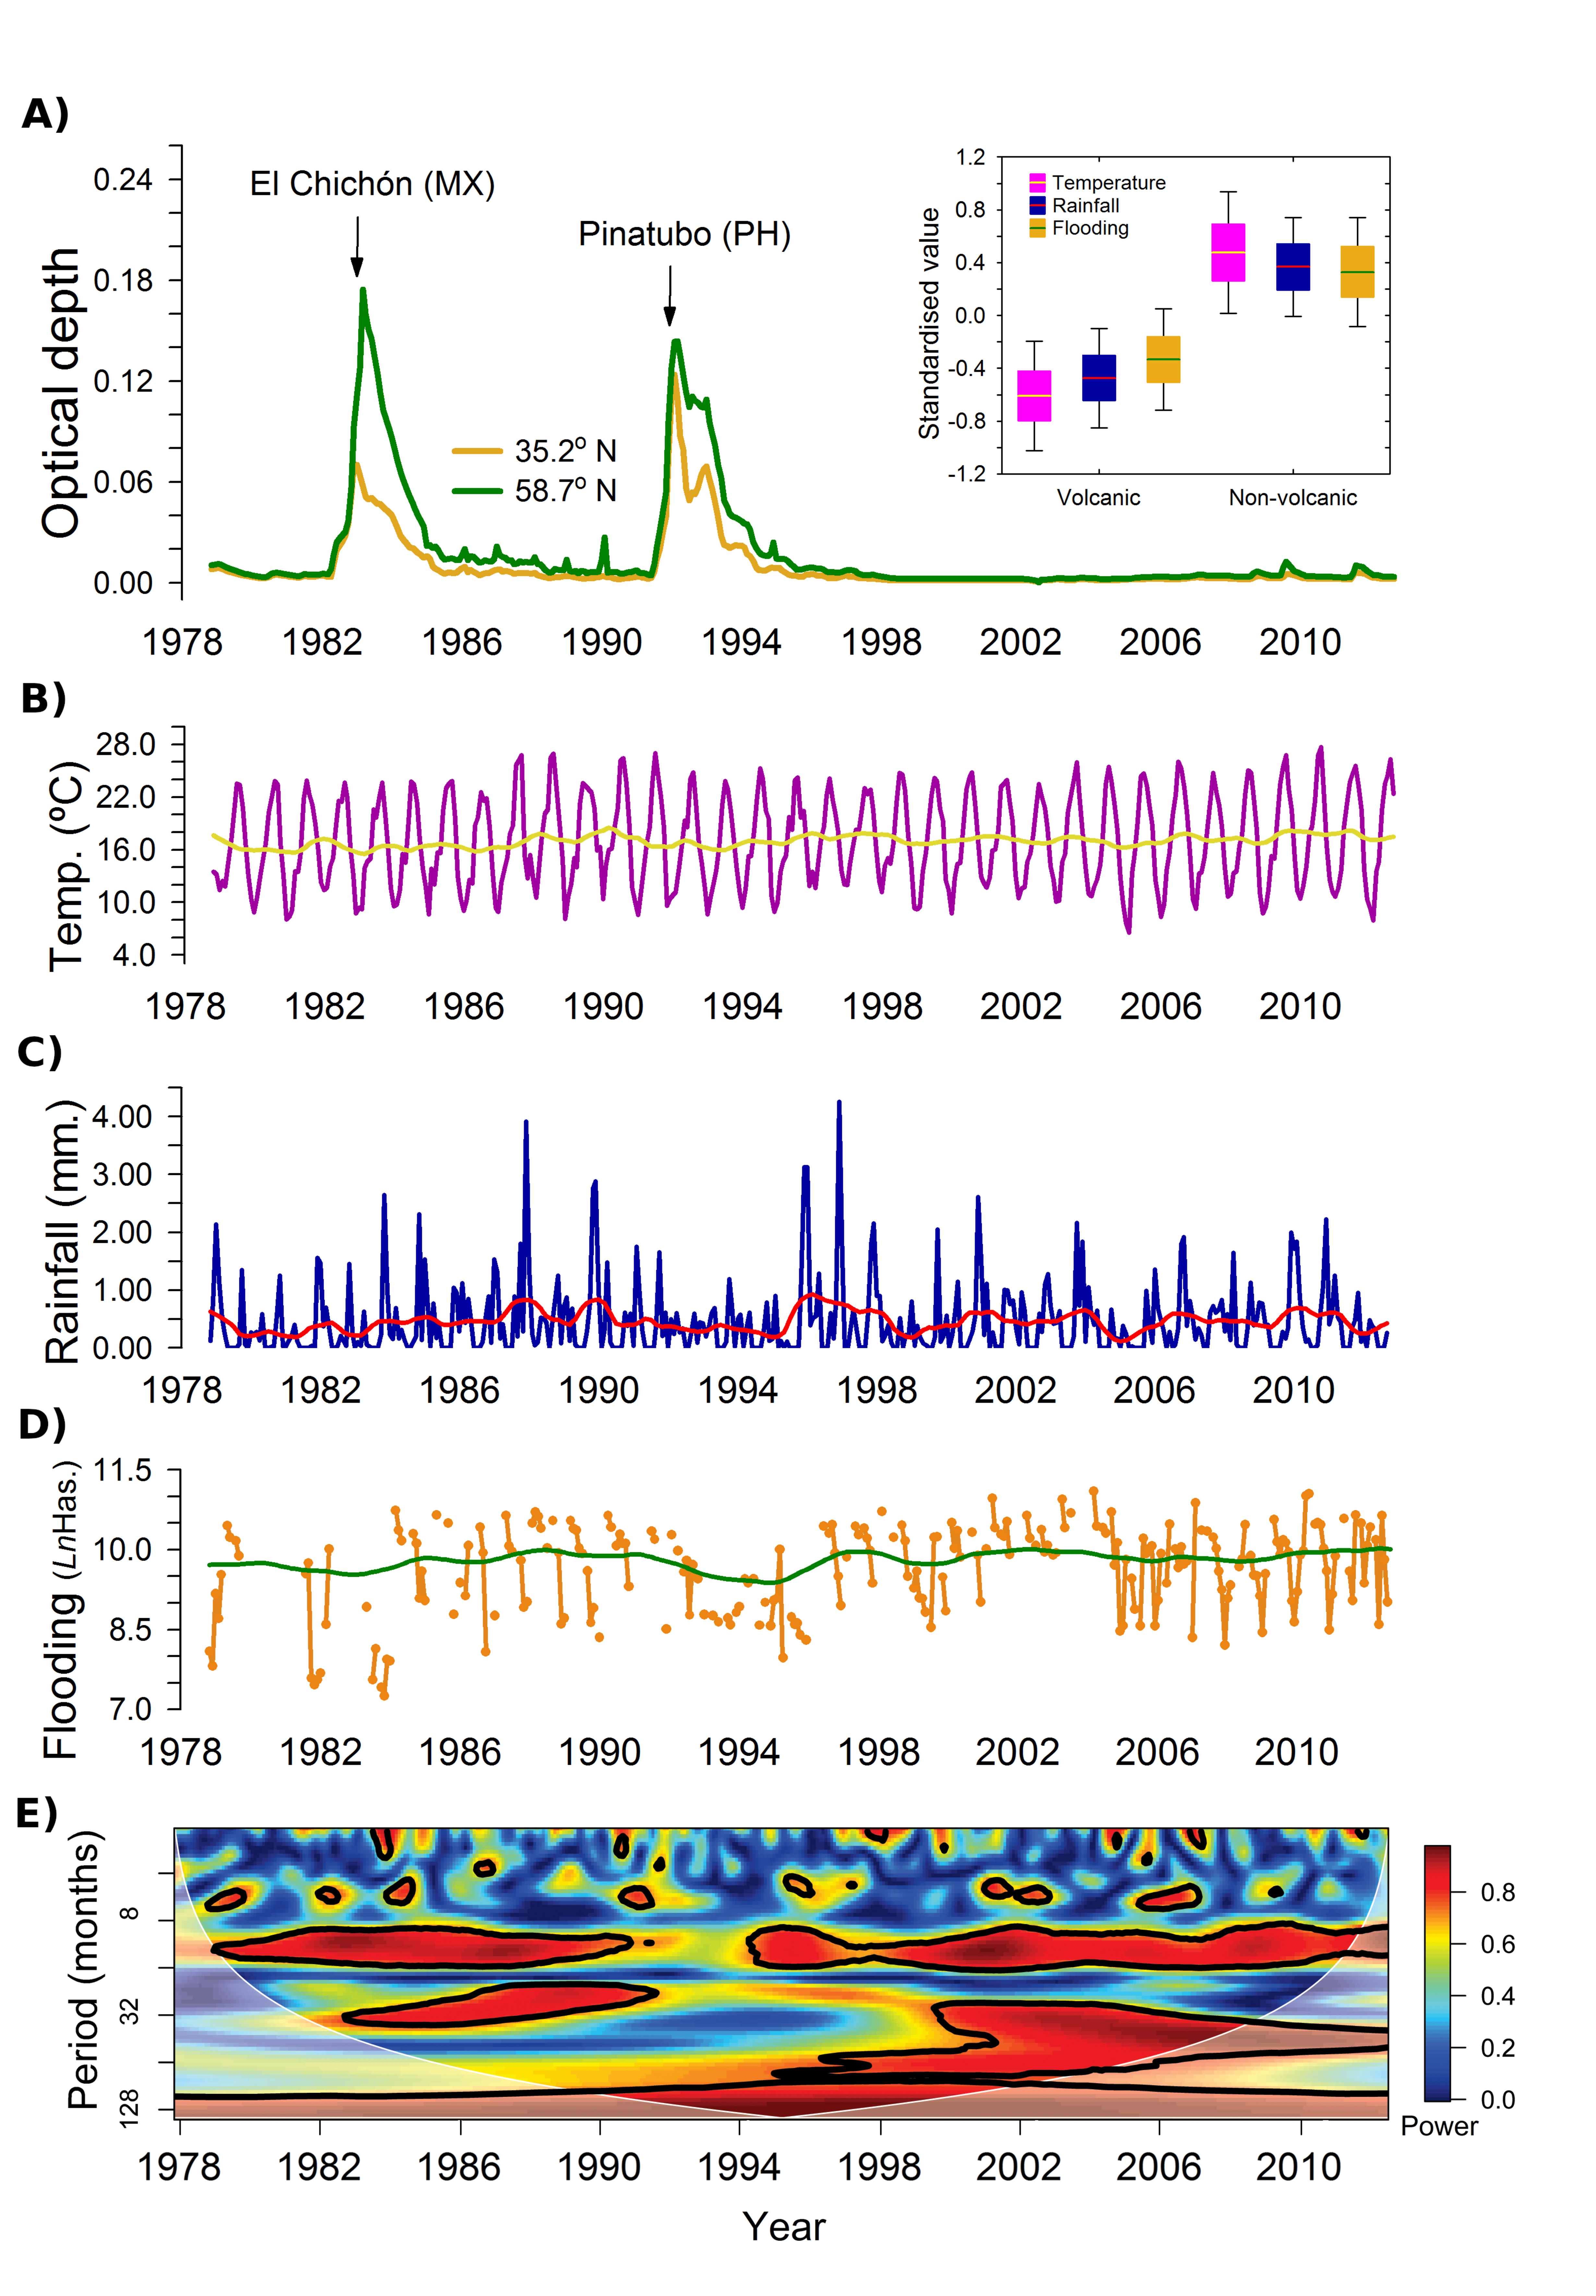
\includegraphics[width=0.6\linewidth]{processed_figs/Environ_clim_ts}
		\caption[Environmental and stratospheric aerosol optical depth time series]{Temporal evolution at monthly steps of the environmental variables used in this study. \textbf{A)} Time series for the stratospheric aerosol optical depth (adim.) in the Northern hemisphere, in yellow and green at two different latitudes (\cite{Booth2012}). The massive stratospheric aerosol injection events of the two largest volcanic eruptions of the study period, El Chichón (Mexico) and Mt. Pinatubo (Philippines), are located with arrows. The inset figure shows the box-plots for the average (horizontal line within each box), Standard Error (Box size) and Standard Deviation (whiskers) of the standardized variables of temperature, precipitation and spatial flooding extension, during volcanic years (1982-1983 and 1992-1995) and non-volcanic years. \textbf{B)} Monthly time series of temperature ($^\circ \mathrm{C}$) in the study area (\cite{Almaraz2012}, in purple), with smoothed loess fitting in yellow. \textbf{C)} Rainfall (mm.) in the study area in blue, with smoothed loess fitting in red. \textbf{D)} Spatial flooding extension (\textit{Ln}Has.) in the Doñana wetlands, including all types of flooded surfaces in orange, with smoothed loess fitting in green. \textbf{E)} Wavelet spectrum for the precipitation time series (\cite{Cazelles2008}). Power values within black contours indicate statistically significant periodicity.}
		\label{fig:StructChanFullDoniana}
	\end{figure}
	
	\begin{figure}[t]
		\centering
		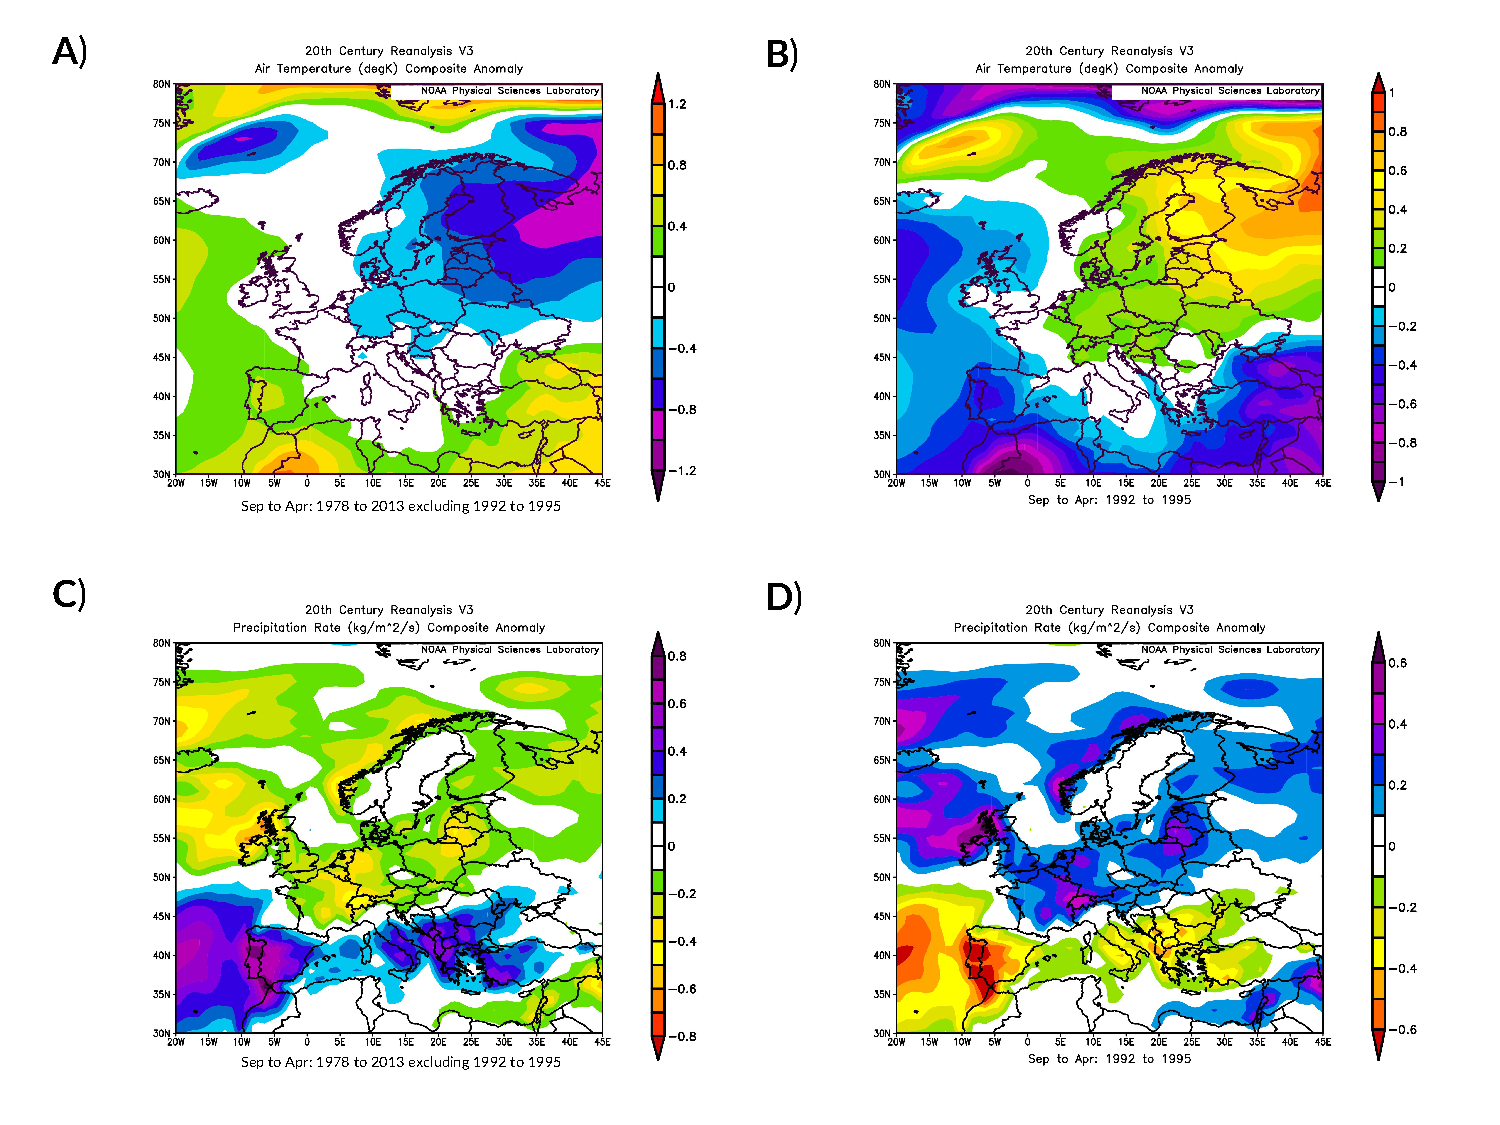
\includegraphics[width=\linewidth]{processed_figs/NOAA_CAR.pdf}
		\caption[Synoptic fields of composite anomalies obtained from the V3 of the Twentieth Century Reanalysis Project]{Synoptic fields of composite anomalies obtained from the V3 of the Twentieth Century Reanalysis Project (\url{https://psl.noaa.gov/data/20thC_Rean/}). The composite anomaly from 1978 to 2013, excluding the transient period 1992-1995, is shown for air temperature (\textbf{A}) and precipitation rate (\textbf{C}). The composite anomaly for the transient period, 1992-1995, is shown for air temperature (\textbf{B}) and precipitation rate (\textbf{D}). The seasonal period considered excludes the summer months. }
		\label{fig:CRP_NASA_V3}
	\end{figure}
	
	\begin{figure}[t]
		\centering
		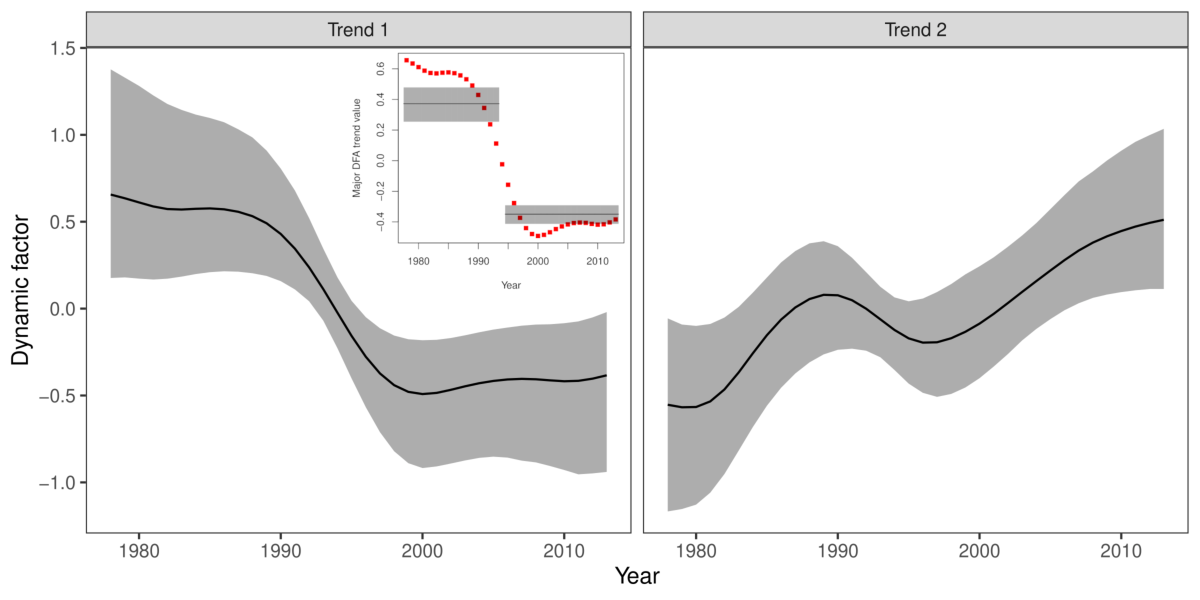
\includegraphics[width=1\linewidth]{processed_figs/Common_Trends}
		\caption[Posterior estimated community common DFA trends]{Posterior estimated community common trends in abundance of the state-space Dynamic Factor Analysis (\cite{Ward2022}) applied to the wintering waterfowl community, and 95 \% credible intervals. The inset figure in the common trend 1 shows the posterior regime shift identified by a Hidden Markov Model applied to the first common trend of the state-space DFA. The values of the common trend are depicted as red axes, and the average (and 95\% Credible Intervals) of each regime is denote in gray.}
		\label{fig:Common_Trends}
	\end{figure}
	
	\begin{figure}[t]
		\centering
		\includegraphics[width=1\linewidth]{../output/figures/Common_Trends_by_Species.pdf}
		\caption[Posterior estimated common trends of the state-space DFA]{Posterior estimated common trends of the state-space Dynamic Factor Analysis for each wintering waterfowl species in Doñana wetlands, 1978-2021. The red dots denote the aerial count estimate for December and January of each wintering season. The solid line is the average posterior value of the common trend in Figure \ref{fig:Common_Trends} yielding the largest factor loading for each species (Figure \ref{fig:Factor_loadings}), and the shaded region is 95 \% credible intervals.}
		\label{fig:Common_Trends_by_Species}
	\end{figure}
	
	\begin{figure}[t]
		\centering
		\includegraphics[width=1\linewidth]{../output/figures/Factor_loadings.pdf}
		\caption[Factors loadings of the state-space DFA]{Factors loadings of the state-space Dynamic Factor Analysis for each wintering waterfowl species and each dynamic common trend (shown in Figs. \ref{fig:Common_Trends} and \ref{fig:Common_Trends_by_Species}). Violin plots include the posterior density for each loading and species, and the gray shading (prob diff0) is proportional to the probability that the loading is different from 0.}
		\label{fig:Factor_loadings}
	\end{figure}
	
	\begin{figure}[t]
		\centering
		\includegraphics[width=\textwidth]{../output/figures/Wrapped_stability}
		\caption[Posterior distribution of dynamical stability and feasibility in alternative stable states]{Probability of dynamical stability and feasibility of the wintering waterfowl community in Doñana marshes (1978-2013). Figures \textbf{A}) and \textbf{B}) show the distribution in the unit circle of the posterior eigenvalues of the Jacobian matrix \ref{LVR_Jacobian_RS} of the LVR state-space model (Eqns. \ref{LVR_State_Equation_form}-\ref{LVR_Obs_Equation_form}) fitted to the pre-Pinatubo period (\textbf{A}, 1978-1992) and the post-Pinatubo period (\textbf{B}, 1995-2013). The probability of stability is the fraction of the eigenvalues (modulus) strictly smaller than 1 in the posterior distribution. MAP is the maximum a posteriori density, and 90\% HDI the highest density interval (\cite{Makowski2019}). Figures \textbf{C}) and \textbf{D}) show the posterior histograms of the equilibrium abundances ($N^*$) and the posterior averages of the carrying capacities, $k_{i}$ (Eqn. \ref{LVR_State_Equation_form}), for each waterfowl species (red dots) in the pre-Pinatubo period (\textbf{C}) and the post-Pinatubo period (\textbf{D}). The probability of feasibility for each period is the proportion of posterior estimated equilibrium abundance vectors in which the abundances are strictly positive for all species.}
		\label{fig:Wrapped_stability}
		% \setfloatalignment{b}  %b/t
		% \forceversofloat  % \forcerectofloat
	\end{figure}
	
	\begin{figure}[t]
		\centering
		\includegraphics[width=0.7\linewidth]{../output/figures/Prob_of_extinction}
		\caption[Change in probability of species extinction between two periods]{Change in the estimated probability of extinction at equilibrium for each waterfowl species in Doñana wetlands before (purple dots) and after the eruption of Mt. Pinatubo (green dots). From the posterior of the Bayesian regime-dependent state-space LVR model (Eqns. \ref{LVR_State_Equation_form}-\ref{LVR_Obs_Equation_form}) fitted to the time-series of community abundance, this probability is calculated, for each species and alternative stable state, as the fraction of posterior estimated population abundances at equilibrium that are not strictly positive. Note the \textit{sqrt}-transformation of the \textit{x}-axis.}
		\label{fig:Extinction}
	\end{figure}
	
	\begin{figure}[t]
		\centering
		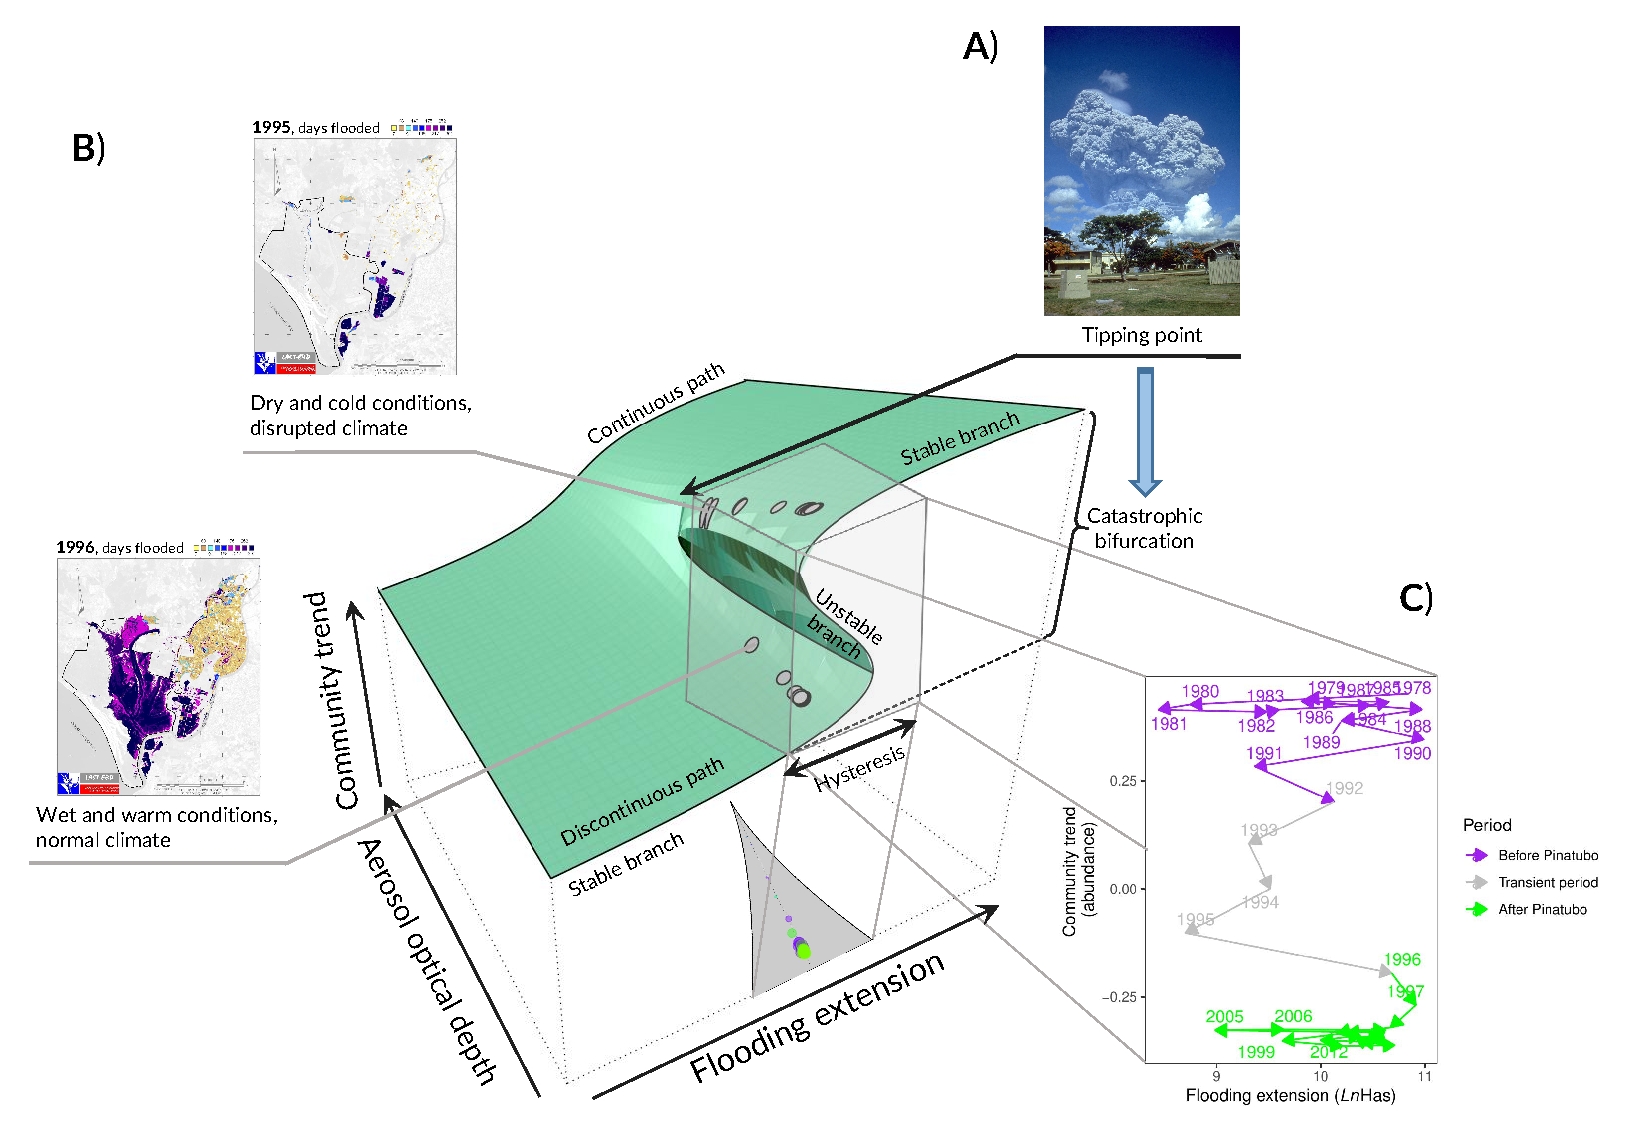
\includegraphics[width=\linewidth]{processed_figs/Cusp_diagram}
		\caption[Three-dimensional diagram of the fitted stochastic cusp catastrophe model]{{\scriptsize\setstretch{1} Diagram depicting the three-dimensional representation of the stochastic cusp catastrophe model (Eqn. \ref{Cusp_Final}) fitted to the major community trend (\textit{z}-axis, Trend 1 in Fig. \ref{fig:Common_Trends}), as a function of the stratospheric aerosol optical depth (bifurcation parameter) and flooding extension (asymmetry parameter). The fitted values plotted in the maximum-likelihood cusp equilibrium surface (in green) are depicted as gray circles. In \textbf{A}), the tipping point (the cusp) of the model is represented by the eruption of Mt. Pinatubo of Philippines in April 2, 1991. As a press-type perturbation, it triggered a transient period of dry and cold wintering conditions in the Southern Palaearctic that lasted until 1995 (\cite{Robock2002}). Before the tipping point, fluctuations in waterfowl community abundance were located in the upper stable branch of the surface. In \textbf{B}), the small figures show maps of the numbers of days of flooded conditions in Doñana wetlands for two distinct years: 1995, at the end of transient period characterized by dry and cold wintering conditions; and 1996, a climatically normal year, with wet and warm conditions (see Fig. \ref{fig:CRP_NASA_V3}). The dynamic in year 1995 was evolving in the unstable (transient) branch of the surface. From 1996 onwards, the dynamics settled in the lower stable branch. The magnitude of the catastrophic bifurcation triggered by the tipping point is thus the difference in height between the two stable branches, while the size of the region of hysteresis is the amplitude of the stable states of waterfowl community abundance sharing the same environmental conditions. The gray cube in \textbf{B}), with height equal to the size of the catastrophic bifurcation, and width equal to the size of the hysteresis region, contains all the dynamics of the system, that takes place along the discontinuous paths. The bifurcation set is projected as a gray shadow in the floor of the cusp 3D surface, with the cusp as a critical point in the vertex. This set is represented in 2-dimensions in \textbf{C}), were the implicit temporal dynamics of the community abundance trend evolves with respect to the asymmetry parameter, namely flooding extension, from the first stable state (purple arrows) to the second stable state (green arrows) through the transient, unstable period (gray arrows). Flooding data provided by the \href{http://www.ebd.csic.es/web/last/inicio}{LAST-EBD}; Pinatubo public domain image from \href{https://commons.wikimedia.org/wiki/File:Pinatubo_Ausbruch_1991.jpg}{Richard P. Hoblitt, USGS.}}}
		\label{fig:Cusp_Surface}
	\end{figure}

\end{document}